\documentclass[conf]{new-aiaa}
%\documentclass[journal]{new-aiaa} for journal papers
\usepackage[utf8]{inputenc}

% template packages
\usepackage{graphicx}
\usepackage{amsmath}
\usepackage[version=4]{mhchem}
\usepackage{siunitx}
\usepackage{longtable,tabularx}
\setlength\LTleft{0pt} 

% graphics packages
% \usepackage{graphicx}

% algorithm packages
\usepackage{algpseudocode}
\usepackage{algorithm}
\usepackage{amsmath}

% symbols
\usepackage{gensymb}

% reference packages
\usepackage{cleveref}

% formatting packages
% \usepackage[parfill]{parskip}
% \setlength{\parindent}{0cm}
% \usepackage[margin=1in]{geometry}
\usepackage{subfigure}

% editing packages
\usepackage{todonotes}

\title{LES Validation of Wind Farm Layout Optimization Using a Simple Wake Model and Gradient-Based Optimization}

\author{Jared J. Thomas\footnote{PhD Student, Department of Mechanical Engineering, 360 EB, Provo, UT 84602, AIAA Student Member}}
\affil{Brigham Young University, Provo, UT 84602}
\author{Jennifer Annoni \footnote{Research Engineer, National Wind Technology Center, 15013 Denver W Pkwy, Golden, CO 80401.}}
\author{Paul Fleming \footnote{Senior Engineer, National Wind Technology Center, 15013 Denver W Pkwy, Golden, CO 80401.}}
\affil{National Renewable Energy Laboratory, Golden, CO, 80401, USA}
\author{Andrew Ning\footnote{Assistant Professor, Department of Mechanical Engineering, 360 EB, Provo, UT 84602, AIAA Senior Member}}
\affil{Brigham Young University, Provo, UT 84602}

\begin{document}

\maketitle

% \begin{abstract}
% These instructions give you guidelines for preparing papers for AIAA Technical Papers using \LaTeX{}. Define all symbols used in the abstract. Do not cite references in the abstract. The footnote on the first page should list the Job Title and AIAA Member Grade for each author, if known Authors do not have to be AIAA members.
% \end{abstract}


\section{Introduction}

%For an extensive review of the area, refer to Herbert-Acero et al. (2014) \cite{acero2014}. 
 Wind farm layouts are typically optimized using gradient-free optimization methods. However, grandient-free optimization methods exhibit reduced performance when applied to high dimensional problems \cite{rios2013-grad-free-comparison}. In \cite{rios2013-grad-free-comparison}, most gradient-free solvers were unable to solve more than $15\%$ of the test problems studied with 10-30 design variables, while the best methods tested could solve only $28\%$ of the test problems with 31-300 design variables. The wind farm layout optimization problem (WFLOP) certainly falls into this category, with each turbine requiring at least two additional design variables for free design space exploration. New wind farms can include well over 100 turbines, meaning  over 200 variables and thousands of constraints. In short, the variables and constraints of the WFLOPs of interest exceed the abilities of gradient-free optimization methods.

In contrast to gradient-free optimization methods, some gradient-based methods can solve problems with thousands of variables and constraints \cite{gill2005}. However, gradient-based methods are prone to premature convergence when used with multi-modal problems, such as the WFLOP \cite{acero2014}. Because of the tendency to converge to local optima in multi-modal problems, gradient-based optimization methods have not historically been seen as viable for solving the WFLOP. However, recent studies have demonstrated that significant improvements to wind farm layouts, if not global optimality, can be obtained by using gradient-based methods either alone \cite{fleming2015, guirguis2016, gebraad2017-max-aep, thomas2017, thomas2018-wec},  or with gradient-free methods in a hybrid approach \cite{rethore2014}. 

While the recent results to WFLOPs obtained using gradient-based optimization are promising, it is important to confirm that improvements obtained during optimization are not merely artifacts of the simplified models being used during optimization. Comparing various layouts within a single wind farm is problematic. It is unrealistic to build a wind farm multiple times to test various designs, so we are left with wind tunnel testing and large eddy simulations (LES). In this work we have validated the optimized results using LES.

Solving a WFLOP requires several different types of models. Two of the most important of these are the wake model and the farm model. Generally speaking, wind turbine wake models define the wind speed in a turbine wake given a set of inflow conditions, while farm models combine the wakes of various turbines to determine the cumulative effects of the wakes of multiple turbines. Many different wind turbine wake and wind farm models have been presented, all with varying levels of accuracy and computational cost. Many of the wake models, such as the ``tophat" Jensen/Park model \cite{jensen1983}, the Frandsen model \cite{frandsen2006}, and the original FLORIS model \cite{gebraad2014}, have regions of non-physical zero-valued gradients, where their gradients go to zero while the gradients of the real design space do not. If a model with non-physical zero-valued gradients is used with gradient-based optimization, the optimization may converge to an especially poor local optimum due to the lack of information provided in the gradients \cite{thomas2017}.

The Bastankhah and Port\'{e}-Agel (BP) wake model presented in \cite{bastankhah2014, bastankhah2016} is well suited to gradient-based optimization, with the exception of the near wake region. Most of the BP model is smooth, continuous, and free from flat regions, but the near wake defition of the BP model can be either flat or undefined. The near wake region is rarely needed for evaluating a wind farm since wind turbines are usually placed far enough from each other that they are in the far wake. While the final wind farm design may not place turbines in the near wake, it is important to have the near wake region defined and non-flat during gradient-based optimization because optimization algorithms may attempt infeasible solutions during the optimization process \cite{belegundu2011} and the near wake region of the BP model may not be outside the defined optimization constraints. The BP wake model uses a Gaussian distribution to define the rest of the wake, and is easily applied to different turbines since it only has one independent parameter. Building on the BP wake model, Niayifar and Port\'{e}-Agel (NP) have proposed a farm model \cite{niayifar2015, niayifar2016} to be used in concert with the BP wake model as published in 2014 that also makes the one independent variable dependent on turbulence intensity \cite{bastankhah2014}, though newer version of BP wake model was published in 2016 \cite{bastankhah2016}. In this study we use the NP farm model with the 2016 version of the BP wake model. While the NP model seems to provide good agreement with LES data, there are some minor problems with the NP farm model for use with gradient-based optimization that need to be addressed.

In this work, we address the lack of near wake definition in the BP wake model for the purposes of using gradient-based optimization methods to solve the WFLOP. We then apply the NP wind farm model with some adjustments and obtain exact gradients across the entire system. Finally, we solve the WFLOP using a gradient-based approach and demonstrate the validity of the optimized result using LES.

\section{Methods}

\subsection{Wake Model}
While the BP wake model exhibits many characteristics necessary for use with gradient-based optimization, there are some small issues that must be overcome. First, the main BP model is undefined from the turbine location up to several diameters downstream of the the wind turbine. Bastankhah and Port\'{e}-Agel suggested using a constant velocity in this region \cite{bastankhah2016}, but using regions of constant velocity in the wind turbine wake has been shown to cause premature convergence to very poor local optima when optimizing with gradient-based methods \cite{thomas2017}. The standard BP model cannot be used in the near-wake region because there is a discontinuity due to a negative value in the square-root term of the velocity deficit calculation of the BP wake model as shown in \cref{eq:bp-vel}. \todo{double check all equations}
\begin{equation}\label{eq:bp-vel}
	\frac{\Delta \bar{u}}{\bar{u}_{i}} = \Bigg[1-\sqrt{1-\frac{C_{T} \cos{\gamma}}{8 \sigma_y \sigma_z/d^2}}~\Bigg] \exp{\bigg(-0.5\bigg[\frac{y-\delta}{\sigma_y}\bigg]^2\bigg)}\exp{\bigg(-0.5\bigg[\frac{z-z_h}{\sigma_z}\bigg]^2\bigg)}
\end{equation}
%
Where $\Delta\bar{u}$ is the average velocity deficit in the wake due to turbine $i$ at the point of interest, $\bar{u}_{i}$ is the average inflow velocity of turbine $i$, $C_T$ is the thrust coefficient, $\gamma$ is the yaw relative to the inflow wind direction, $d$ is the rotor diameter, $y$ is the horizontal distance from the line through the rotor hub to the point point of interest perpendicularl to the wind direction, $\delta$ is horizontal wake offset, $z$ and $z_h$ are the hights of the point of interest and the rotor hub respectively, and $\sigma_y$ and $\sigma_z$ are the horizontal and vertical wake spread as defined in \cref{eq:sigmay,eq:sigmaz}.
%
\begin{equation}\label{eq:sigmay}
	\sigma_y = k_y [x - x_0] + \frac{d \cos{\gamma}}{\sqrt{8}}
\end{equation}
%
%
\begin{equation}\label{eq:sigmaz}
	\sigma_z = k_z [x - x_0] + \frac{d}{\sqrt{8}}
\end{equation}
%
where $k_y$ and $k_z$ are the herizontal and vertical wake growth rates (assumed to be equal), $x$  is the downstream distance from the turbine, $x_0$ is the length of the potential core as defined in \cref{eq:potentialcore}.
%
\begin{equation}\label{eq:potentialcore}
	\frac{x_0}{d} = \frac{\cos{\gamma }\Big[1+\sqrt{1-C_T}\Big]}{\sqrt{2} \Big[\alpha ^* I + \beta ^* \Big[1- \sqrt{1-C_T}\Big]\Big]}
\end{equation}
where $I$ is the turbulence intensity, $\alpha^*=2.32$, and $\beta^*=0.154$. The discontinuity can occur for various combinations of $k_y$, $k_z$, and $(x-x_0)$. When local turbulence intensity is calculated in the NP wind farm model, as in \cite{niayifar2016} (discussed further in \cref{sec:npa}), the values of $k_y$ and $k_z$ vary and so the discontinuity is even more mobile than in the original model. We can determine where the model is undefined as follows. First, we know the model is undefined when
%
\begin{equation}
	\frac{C_T \cos{\gamma}}{8\sigma_y \sigma_z/d^2} > 1
\end{equation}
%
By substituting in from \cref{eq:sigmay,eq:sigmaz}, and separating the terms based on the powers of $[x-x_0]$, we obtain
%
\begin{equation}
	k_y k_z [x-x_0]^2 + \frac{d[k_y+k_z \cos{\gamma}]}{\sqrt{8}}[x-x_0] - \frac{d^2 \cos{\gamma}[C_T -1]}{8} < 0
\end{equation}
%
To find the exact downstream location where the model begins to be defined, $x_d$, we apply the quadratic formula, select the relevant root, and then solve for $x$ to obtain
%
\begin{equation}\label{eq:xd}
	x_d \leq x_0 + \frac{d\Big[k_y+k_z\cos{\gamma} - \sqrt{[k_y+k_z\cos{\gamma}]^2-4k_y k_z[C_T-1]\cos{\gamma}}\Big]}{2k_y k_z\sqrt{8}}
\end{equation}
%
The model, then, is undefined for regions where $x<x_d$. 

\vspace{5mm}

To remove the discontinuity, we used linear interpolation on both the velocity value and the wake spread. First, the magnitude of the Gaussian curve at $x_d$ is calculated as follows
%
\begin{equation}
	\Delta V_{d,m} = 1 - \sqrt{1 - \frac{C_T \cos{\gamma}}{8 \sigma_{y,d}  \sigma_{z,d}/D_r^2}}
\end{equation}
%
Then, using the magnitude of the Gaussian curve, and keeping the wake spread constant for the velocity calculation, the normalized velocity difference is calculated as a function of the downstream position of the point of interest ($x$)
\begin{equation}
	\Delta V = \bigg[x\bigg[\frac{\Delta V_{d,m} - \Delta V_r}{x_d}\bigg] + \Delta V_r\bigg]
        \exp{\bigg(-0.5  \bigg[\bigg[\frac{\Delta Y }{ \sigma_{y,d}}\bigg]^2+\bigg[\frac{\Delta Z }{ \sigma_{z,d}}\bigg]^2~\bigg]\bigg)}
\end{equation}
%
where $\Delta V_r$ is a pre-determined normalized velocity deficit at the rotor hub. We used a value of $\Delta V_r=\Delta V_{d,m}$. With the linear interpolation method, optimizations succeed even when turbines are placed less than one diameter from each other.
\todo{transition}
Wind shear was added to the model using a power law defined as
%
\begin{equation} \label{eq:shear}
	u = u_r\bigg[\frac{z-z_o}{z_r-z_o}\bigg]^\psi
\end{equation}
%
where $u_r$ is the reference wind speed, $z$ is the height of interest, $z_r$ is the height at which $u_r$ was measured, $z_o$ is the height of local ground, and $\psi$ is the shear exponent. The value of $\psi$ for comparison to the LES was determined by fitting \cref{eq:shear} to a series of wind speeds in the LES precursor used for validation. To fit the curve, $z_r$ was set to 80 m. The appropriate value of $\psi$ for comparison to the LES was determined to be 0.31.
%0665565.
The shear exponent fitting plot can be seen in \cref{fig:shear_fit}
%
\begin{figure}[ht]
	\centering
	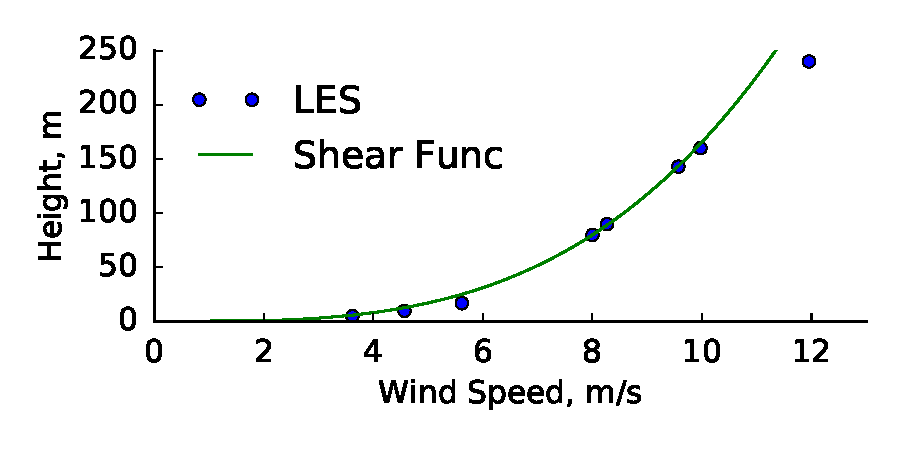
\includegraphics[width=0.75\textwidth]{final_images/shear_fit.pdf}
	\caption{The calculated wind speed using the power law (\cref{eq:shear}) with shear exponent $\psi=0.31$ compared with the values obtained from the LES precursor. The reference values used were a height of 80 m with a wind speed of 8 m/s}
	\label{fig:shear_fit}
\end{figure}
%

The results of the model changes discussed above can be seen in \cref{fig:model_contours}. These changes make the model continuous throughout the domain and differentiable everywhere except at the exact turbine location. With a separation constraint in place, the probability of turbines landing exactly on top of each other is extremely small, as noted in \cite{thomas2017}. While the linear interpolation makes very little attempt to be physically accurate in the near wake, the accuracy of the model for AEP calculation purposes should be unaffected since turbines will almost never be placed close enough together to be in the linear interpolation region in a final design. If greater accuracy is desired in the near wake, it would be feasible to use the linear interpolation during optimization and then switch to a more accurate near wake model for final calculations, such as the one proposed in \cite{keane2016}.

\begin{figure}[htbp!]
	\centering
	\subfigure[]{
		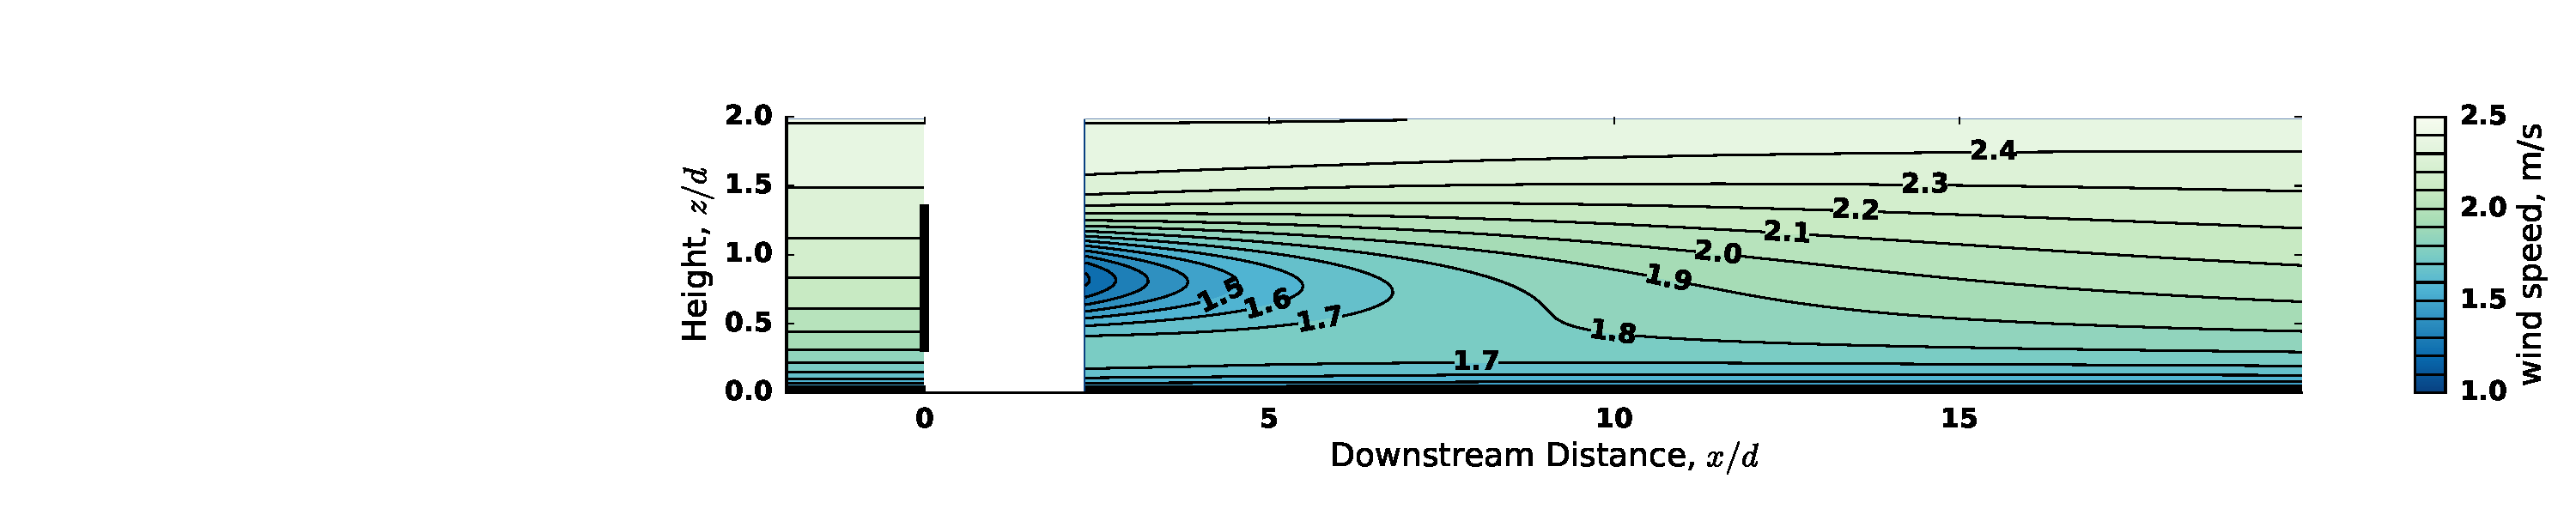
\includegraphics[width=0.75\textwidth, trim={18.5cm 1cm 4.cm 1cm}]{final_images/model_contours_vertical_before.pdf}
	}
	\subfigure[]{
		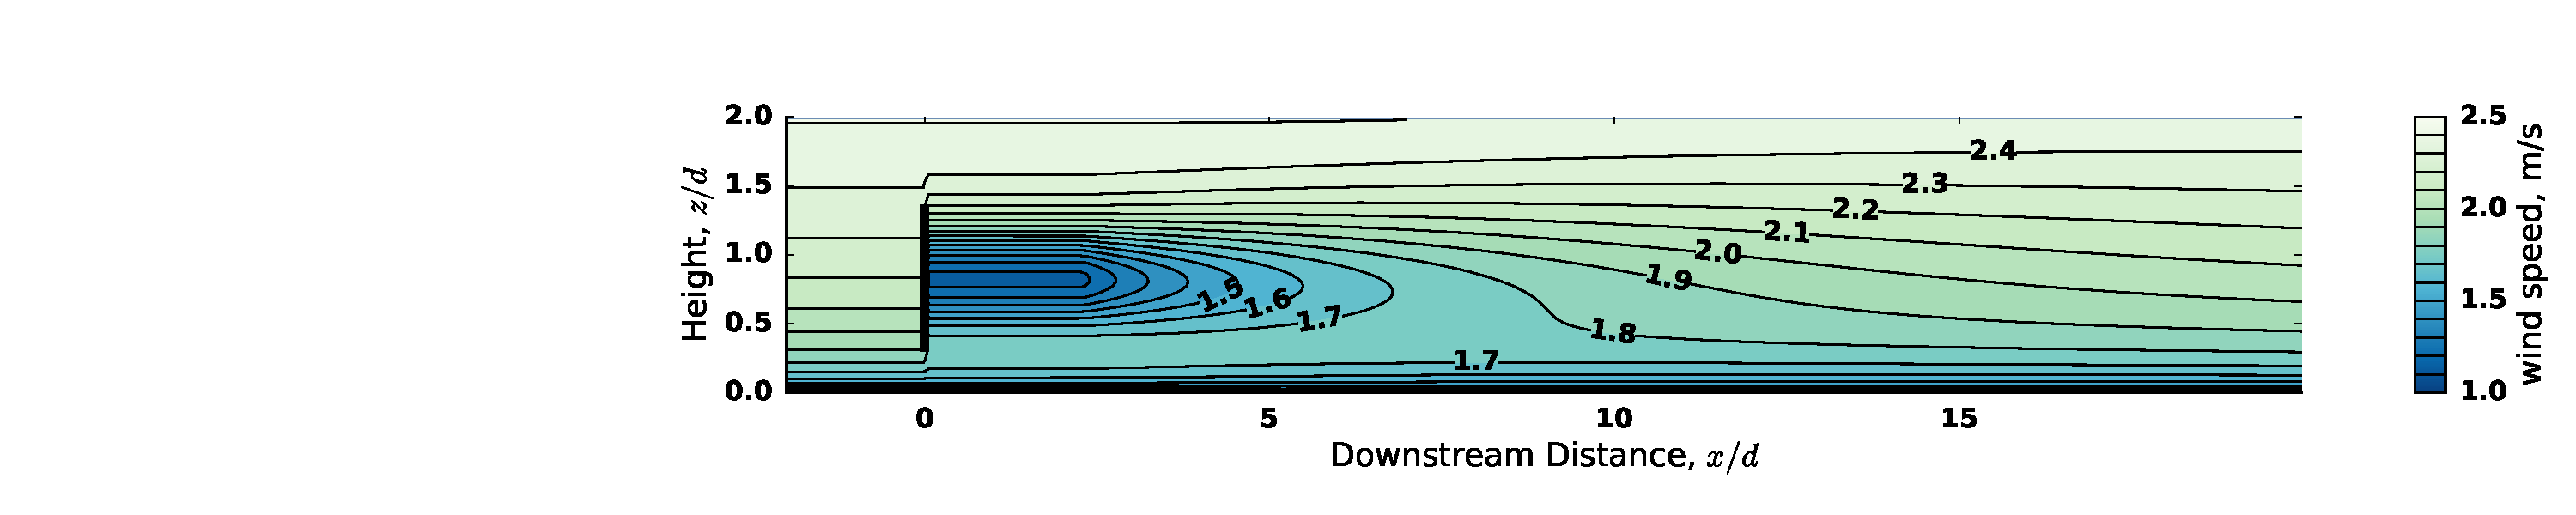
\includegraphics[width=0.75\textwidth, trim={18.5cm 1cm 4.cm 1cm}]{final_images/model_contours_vertical_after.pdf}
	}
	\caption{Bastankhah and Port\'{e}-Agel wake model (a) without and (b) with the added linear interpolation for the near wake and shear model. The heavy black line represents the turbine rotor. This figure was included for comparison with figure 6 of Bastankhah and Port\'{e}-Agel (2014) \cite{bastankhah2014}, and so model values were chosen accordingly (small wind turbine for use in a wind tunnel). We used a shear exponent of 0.15 for this figure.}
	
	\label{fig:model_contours}
\end{figure}

\subsection{Wind Farm Model}\label{sec:npa}
Niayifar and Port\'{e}-Agel proposed a wind farm model that used the Bastankhah and Port\'{e}-Agel model as published in 2014 \cite{bastankhah2014} for calculating the wind speed in the wakes \cite{niayifar2015, niayifar2016}. We applied the same wind farm model to the 2016 version of the Bastankhah and Port\'{e}-Agel model, with some variation as discussed in the following sections.
% However, due to changes made to the Bastankhah and Port\'{e}-Agel wake model published in 2016 \cite{bastankhah2016}, along with the needs of gradient-based optimization, not all of the proposals made by Niayifar and Port\'{e}-Agel in their 2016 paper can be used. This section will discuss which aspects of the Niayifar and Port\'{e}-Agel model that were and were not used in our system.
\subsubsection{Wake Combination}
Niayifar and Port\'{e}-Agel found the most accurate method of wake combination to be a linear interpolation that uses the inflow velocity of the upstream turbine as in \cref{eq:wake-comb-lin}. 
%
\begin{equation}\label{eq:wake-comb-lin}
	\bar{u}_j = \bar{u}_\infty - \sum_{i=1}^{N_T} [\bar{u}_i - \bar{u}_{ij}] = \bar{u}_\infty - \sum_{i=1}^{N_T} [\Delta \bar{u}_{ij}]
\end{equation}
%
Where $\bar{u}_j$ is the inflow velocity at the turbine or point of interest, $U_i$ is the inflow velocity of upstream turbine $i$, $\bar{u}_{ij}$ is the wind speed that would exist at turbine or point $j$ if only turbine $i$ were accounted for, and $\bar{u}_{\infty}$ is the freestream velocity. Our tests of the accuracy of various wake combination methods also found this method to be the most accurate. However, for the upstream turbine velocity to be used, the inflow velocity of the turbines must be calculated in order from upstream to downstream. We used the heapsort algorithm to obtain a sorted index list of the turbines prior to solving the system for each wind direction. Using the sorted index list allowed turbine sorting without over complicating the gradients of the system.

\subsubsection{Turbulence Intensity}
Niayifar and Port\'{e}-Agel calculated local turbulence intensity using the model presented by Crespo and Hern\'{a}ndez in \cite{crespo1996}. The local turbulence intensity is then applied to the Bastankhah and Port\'{e}-Agel model through an empirical model for calculating the wake expansion coefficient as shown in \cref{eq:ti_npa} \cite{niayifar2016}
 %
 \begin{equation} \label{eq:ti_npa}
 	k^* = 0.3837 I + 0.003678
 \end{equation}
%
Where $I$ is the turbulence intensity. This model is only valid for turbulence intensity values between 0.065 and 0.15. While the initial BP wake model does not include turbulence intensity \cite{bastankhah2014}, turbulence intensity was included by Bastankhah and Port\'{e}-Agel in their 2016 version of the model \cite{bastankhah2016}. We used the same turbulence intensity calculations for the BP 2016 wake model as was used for the NP wind farm model. Three different approaches to calculating turbulence intensity were employed at various points in the optimization process. (1) local turbulence intensity with a hard maximum function as done by Niayifar and Port\'{e}-Agel \cite{niayifar2016}, (2) local turbulence intensity with a smooth maximum function, and (3) ambient turbulence intensity only.

The local turbulence intensity calculations proposed by Niayifar and Port\'{e}-Agel \cite{niayifar2016} includes the use of a hard maximum function. The algorithm for calculating local turbulence intensity using the hard maximum function is given in \cref{alg:ti}. In our code implementation, we combined the nested loops used for the velocity and turbulence intensity calculations. 
%
\todo{check the algorithm and update as needed}
\begin{algorithm}
	\caption{Turbulence Intensity Calculation (for more information, see \cite{niayifar2016})}
   \label{alg:ti}
   \begin{algorithmic}
   \Ensure Turbines are sorted by relative downstream position
     \For{$j =  1...N$} \Comment{Downstream turbines}
   	% \State $I_j \gets I_0$ \Comment{Initialize to free-stream turbulence value}
    \State $A_{r_j} \gets \frac{1}{4}\pi D_{r_j}^2$ \Comment{Rotor swept area of turbine $j$}
    \State $I_{+_j} \gets 0$
         \For{$i =  1...N$} \Comment{Upstream turbines}
         	\State $\Delta X \gets x_j - x_i$ \Comment{Turbine separation distance}
         	\If{$\Delta X > 0$}
               \State $\beta \gets 0.5\Big[\Big[1+\sqrt{1-C_{T_i}}\Big]/\sqrt{1-C_{T_i}}\Big]$
               \State $\epsilon \gets 0.2 \sqrt{\beta}$
               \State $\sigma = k_i^*\Delta X+D_{r_i}\epsilon$
               \State $D_w \gets 4\sigma$
               \State $A_{w_{ij}} \gets$ Wake overlap area of wake $i$ and rotor $j$ \Comment{Assume circular wake}
               \If{$C_{T_i} > 0.96$}
                    \State $a_i \gets 0.143 + \sqrt{0.0203-0.6427[0.889 - C_{T_i}]}$ \Comment{Glauert correction\cite{gebraad2017-max-aep}}
               \Else
                   \State $a_i \gets  \frac{1}{2}\Big[1-\sqrt{1-C_{T_i}}\Big]$
               \EndIf
               
               \State $I_{+_{ij}} \gets 0.73 a_{i}^{0.8325} I_i^{0.0325} [\Delta X/D_{r_i}]^{-0.32}$
               \State $I_{+_j} \gets \max{[I_{+_{ij}}A_{w_{ij}}/A_{r_j}, I_{+_j}]}$ \Comment{We used \cref{eq:smoothmax3} during the final optimization}
        	\EndIf
        \EndFor
        \State $I_j \gets \sqrt{I_{0}^2 + I_{+_j}^2}$ \Comment{Directly influenced by only one upstream turbine}
        \State $k_j^* \gets 0.3837I_j+0.003678 $ \Comment{To be used in the wake model calculations}
     \EndFor
   \end{algorithmic}    
\end{algorithm}

Because the hard max creates discontinuites in the model and is not differentiable, we used a smooth maximum function during final optimization. The smooth maximum function we used is shown in \cref{eq:smoothmax1,eq:smoothmax2,eq:smoothmax3} and is derived from the LogSumExp (LSE) function \cite{cook2010-softmaximum}.
%
\begin{equation}\label{eq:smoothmax1}
    t_{max} = \min(t_1, t_2)
\end{equation}
\begin{equation}\label{eq:smoothmax2}
    t_{min} = \max(t_1, t_2)
\end{equation}
\begin{equation}\label{eq:smoothmax3}
   \text{smoothmax}(t_{max},t_{min},s) = \frac{\ln(1+\exp(s[t_{min}-t_{max}]))+s t_{max}}{s}
\end{equation}
%
where $s$ controls the smoothness of the transition between terms and influences the error of the calculation, $t_{max}$ and $t_{min}$ represent the respective maximum and minimum of the two values being compared. In calculating local turbulence intensity, \cref{eq:smoothmax3} is applied as in  \cref{eq:maxti} to compare the product of the added local turbulence intensity and the wake overlap raitio.
%
\begin{equation}\label{eq:maxti}
    I_{+_j} = \text{smoothmax}{\bigg(\frac{I_{+_{ij}}A_{w_{ij}}}{A_{r_j}}\bigg)}
\end{equation}
%
where $A_{w_{ij}}$ is the area of the wake of turbine $i$ at the downstream location of turbine $j$, $A_{r_j}$ is the area of the the rotor of turbine $j$, and $I_{+_{ij}}$ is the added turbulence intensity from turbine $i$ at the downstream location of turbine $j$. In our implementation only two values are compared at a time. The total turbulence intensity is then calculated using \cref{eq:ti_at_turb}
%
\begin{equation}\label{eq:ti_at_turb}
    I_j = \sqrt{I_0^2+I_{+_j}^2}
\end{equation}
%
The maximum error of \cref{eq:smoothmax3} occurs when $t_{min} = t_{max}$, and can be calculated as in \cref{eq:error_max}
%
\begin{equation}\label{eq:error_max}
	Error_{max} = \frac{\ln{(2)}}{s}
\end{equation}
%
To keep the error from the smooth max below 0.001, or about 1\% of the total turbulence intensity, we set $s=700$.

% Using \cref{eq:ti_npa} in the updated wake model would cause the effects of turbulence intensity to be included twice. We used \cref{eq:ti_npa} to estimate the initial $k^*$ only. Within the model itself, the ambient turbulence intensity only impacts the model through Bastankhah and Port\'{e}-Agel (2016) \cite{bastankhah2016} and local turbulence intensity is not calculated. 
%
%Jen changes
% \begin{algorithm}
% 	\caption{Turbulence Intensity Calculation}
%    \label{alg:ti}
%    \begin{algorithmic}
%    \Ensure Turbines are sorted by relative downstream position
%      \For{$j =  1...N$} \Comment{Downstream turbines}
%    	\State $I_{+,j} \gets 0$
%          \For{$i =  1...N$} \Comment{Upstream turbines}
%          	\State $\Delta X \gets x_j - x_i$ 
%          	\If{$\Delta X > 0$}
%                \State $\beta \gets 0.5((1+\sqrt{1-C_{T,i}})/\sqrt{1-C_{T,i}})$
%                \State $\epsilon \gets 0.2 \sqrt{\beta}$
%                \State $\sigma = k_i^*\Delta X+D_{r,i}\epsilon$
%                \State $D_w \gets 4\sigma$
%                \State $A_{w,i,j} \gets$ Wake overlap area of wake $i$ and rotor $j$ \Comment{Circular wake}
%                \State $A_{r,j} \gets \pi D_{r,j}^2/4$ \Comment{Rotor-swept area}
%                \State $I_{+,i,j} \gets 0.73 a_{i}^{0.8325} I_{0,i}^{0.0325} (\Delta X/D_{r,i})^{-0.32}$
%                \State $I_{+,j} \gets \max{((I_{+,i,j}A_{w,i,j}/A_{r,j}), (I_{+,i-1}))}$ \Comment{Discontinuity here}
%         	\EndIf
%         \EndFor
%         \State $I_{0,j} \gets \sqrt{I^2 + I_{+,j}^2}$
%         \State $k_j^* \gets 0.3837I_{0,j}+0.003678 $ \Comment{To be used in the BPA wake model}
%      \EndFor
%    \end{algorithmic}    
% \end{algorithm}
% 

\subsubsection{Sampling Over the Rotor-Swept Area}
Various methods can be used to approximate the effective velocity at the rotor. The ideal method is a full integration across the rotor-swept area. We approximated the integral by sampling the velocity at various points and taking the average. When comparing our code to LES and other data, we used 100 sampling points accross the rotor-swept area arranged in the sunflower seed pattern as shown in \cref{fig:sampling_locs}(a). For efficiency during optimization, we approximated the effective velocity of each wind turbine by using a single sampling point located at the rotor hub as shown in \cref{fig:sampling_locs}(b).

\begin{figure}[ht]
	\centering
	\subfigure[]{
		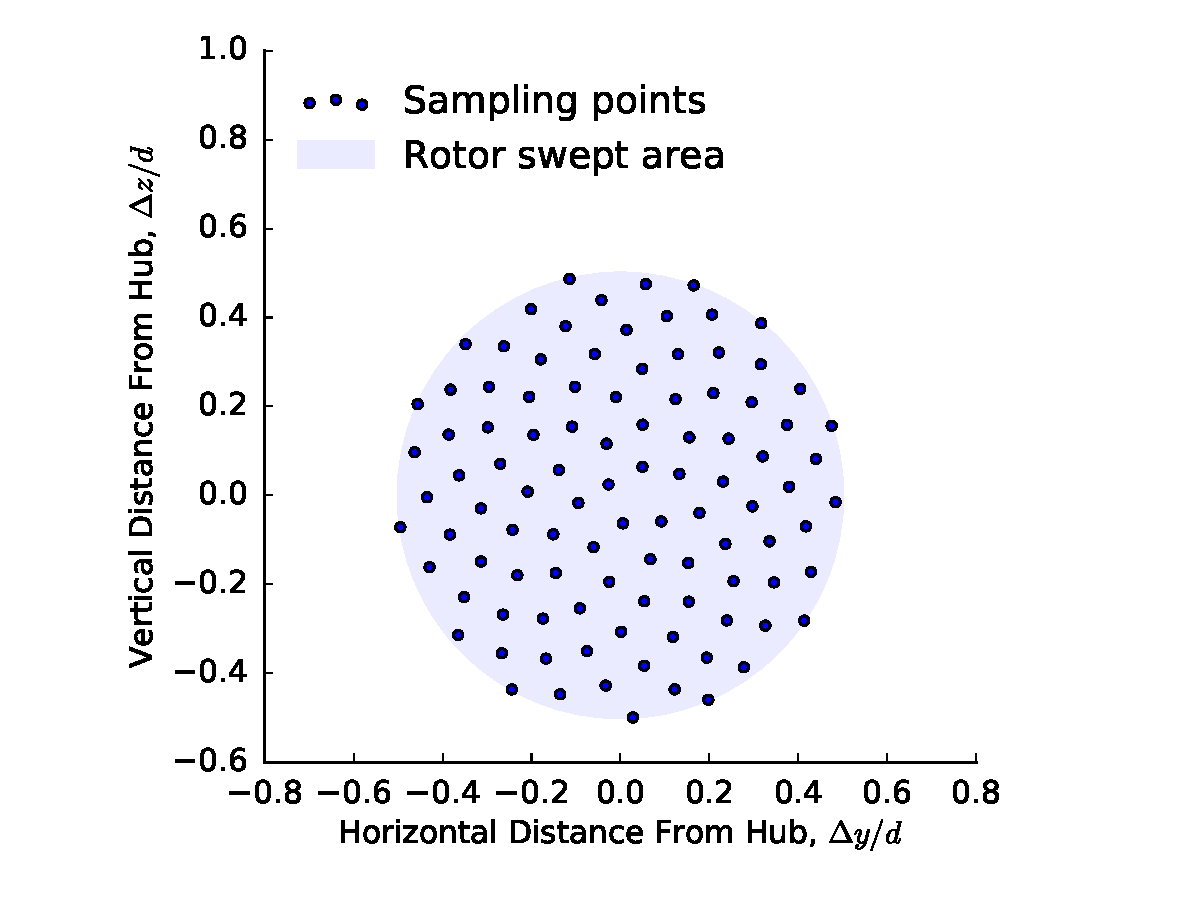
\includegraphics[width=0.48\textwidth, trim={0cm 0cm 0cm 0cm}]{final_images/one_hundred_sampling_points.pdf}
	}
    \subfigure[]{
		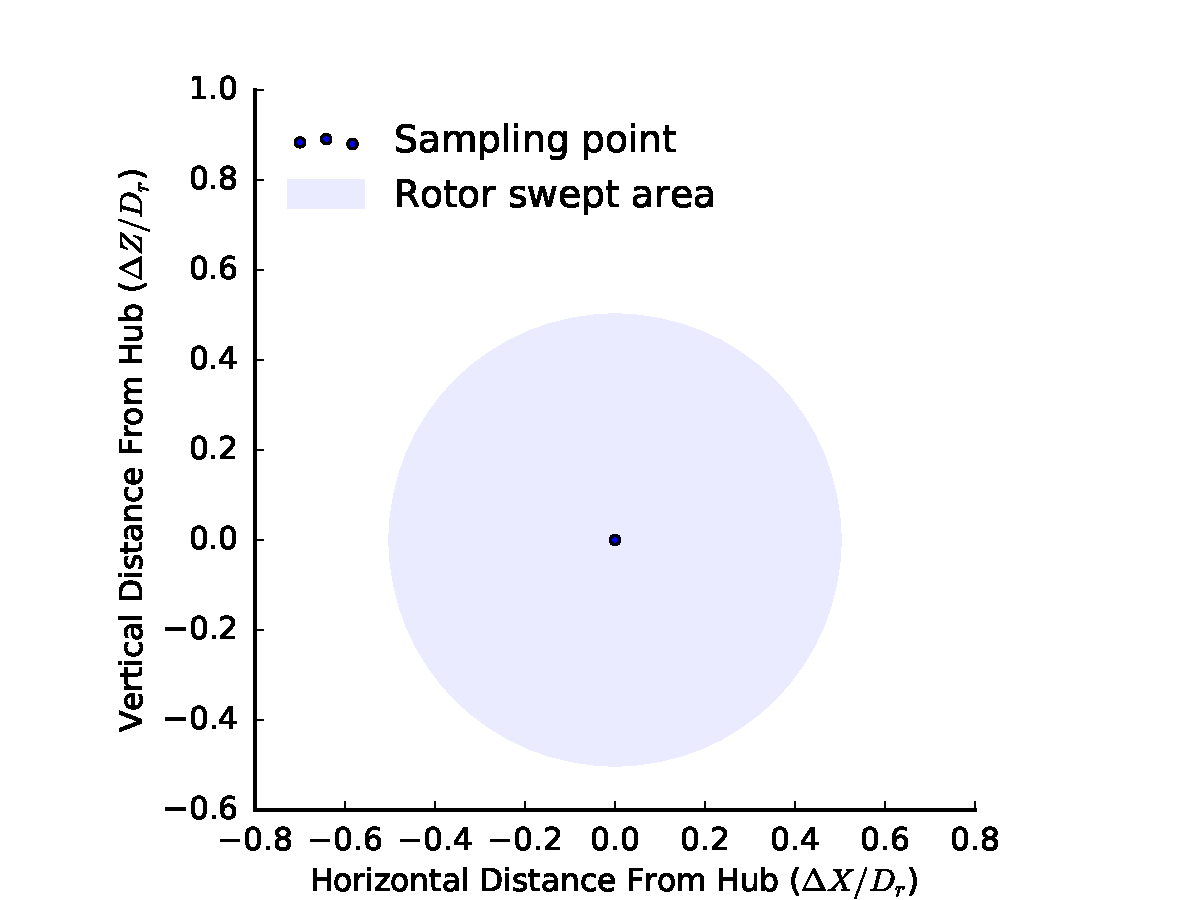
\includegraphics[width=0.48\textwidth, trim={0cm 0cm 0cm 0cm}]{final_images/one_sampling_point.pdf}
	}
% 	\subfigure[]{
% 		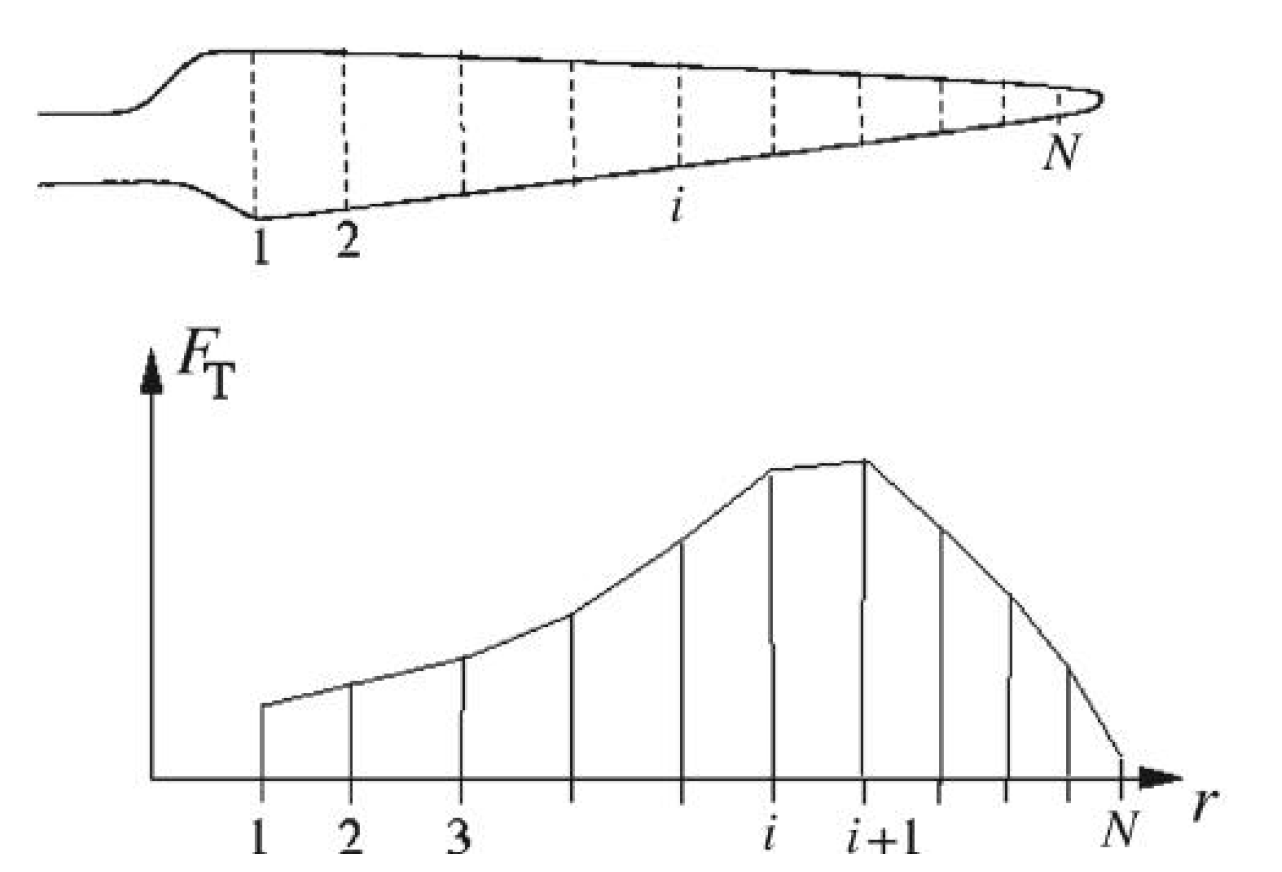
\includegraphics[width=0.43\textwidth, trim={0cm -1cm 0cm 0cm}]{final_images/bem_distribution.png}
% 	}
	\caption{(a) Sampling used to approximate effective hub velocity for LES comparisons. (b) Location of sampling point for approximating effective hub velocity during optimization.}
	\label{fig:sampling_locs}
\end{figure}

\subsubsection{AEP and Wind Turbine Power}
AEP was calculated as in \cref{eq:aep}
\begin{equation}
    \label{eq:aep}
    AEP = \bigg[\frac{hours}{day}\bigg]\bigg[\frac{days}{year} \bigg]\sum_{k=1}^{N_D} \bigg[ f_k \sum_{j=1}^{N_T}P_{j_k} \bigg]
\end{equation}
%
where $N_D$ is the number of wind directions, $N_T$ is the number of wind wind turbines, $f_k$ is the probability of wind in direction $k$, and power of turbine $j$ in direction $k$, $P_{j_k}$, is calculated based on the definition of the power coefficient as done in \cite{gebraad2014} and shown in \cref{eq:power}.
%
\begin{equation}\label{eq:power}
    P_{j_k} = 
    \begin{cases} 
      0 & \bar{u}_j < u_{cutin} \\
      0.5\rho A_j C_{P_j}\bar{u}_j^3 & \bar{u}_j \geq  u_{cutin} \ \text{and} \ P_{j} < P_{rated} \\
      P_{rated} & P_{j} \geq P_{rated}
\end{cases}
\end{equation}
%
where $\rho$ is the air density, $A_j$ represents the rotor-swept area of turbine $j$, and $C_{P_j}$ is the power coefficient of turbine $j$ for the given effective wind speed at the rotor ($\bar{u}_j$).

\subsubsection{Model Verification}
To verify our implimentation of the models described, we compared the output of our code with data for the Horns Rev wind farm from Niayifar and Port\'{e}-Agel \cite{niayifar2016} as shown in \cref{fig:power_line,fig:power_direction}. We calculated error as based on the LES data values from \cite{niayifar2016}. For the Horns Rev row averaging comparison using 100 samples on the rotor-swept area as shown in \cref{fig:power_line}(a): the model values shown by Niayifar and Port\'{e}-Agel had an average error of $6.2\%$ and a maximum error of $10.9\%$; Ignoring local turbulence intensity resulted in an average error of $32.9\%$ and a maximum error of $46.2\%$; calculating local turbulence intensity using either the hard maximum or smooth maximum both resulted in an average error of $3.4\%$ and a maximum error of $6.7\%$.  For the Horns Rev directional power comparison using 100 samples on the rotor-swept area as shown in \cref{fig:power_direction}(a): the model values shown by Niayifar and Port\'{e}-Agel had an average error of $3.0\%$ and a maximum error of $7.5\%$; Ignoring local turbulence intensity resulted in an average error of $8.4\%$ and a maximum error of $34.6\%$; calculating local turbulence intensity using either the hard maximum or smooth maximum both resulted in an average error of $2.2\%$ and a maximum error of $7.1\%$. The high errors when local turbulence intensity is ignored are in the directions of highest wake interactions as can be seen in \cref{fig:power_direction} and do not alter the general trend of the directional power. 

\begin{figure}[htbp!]
	\centering
	\subfigure[]{
		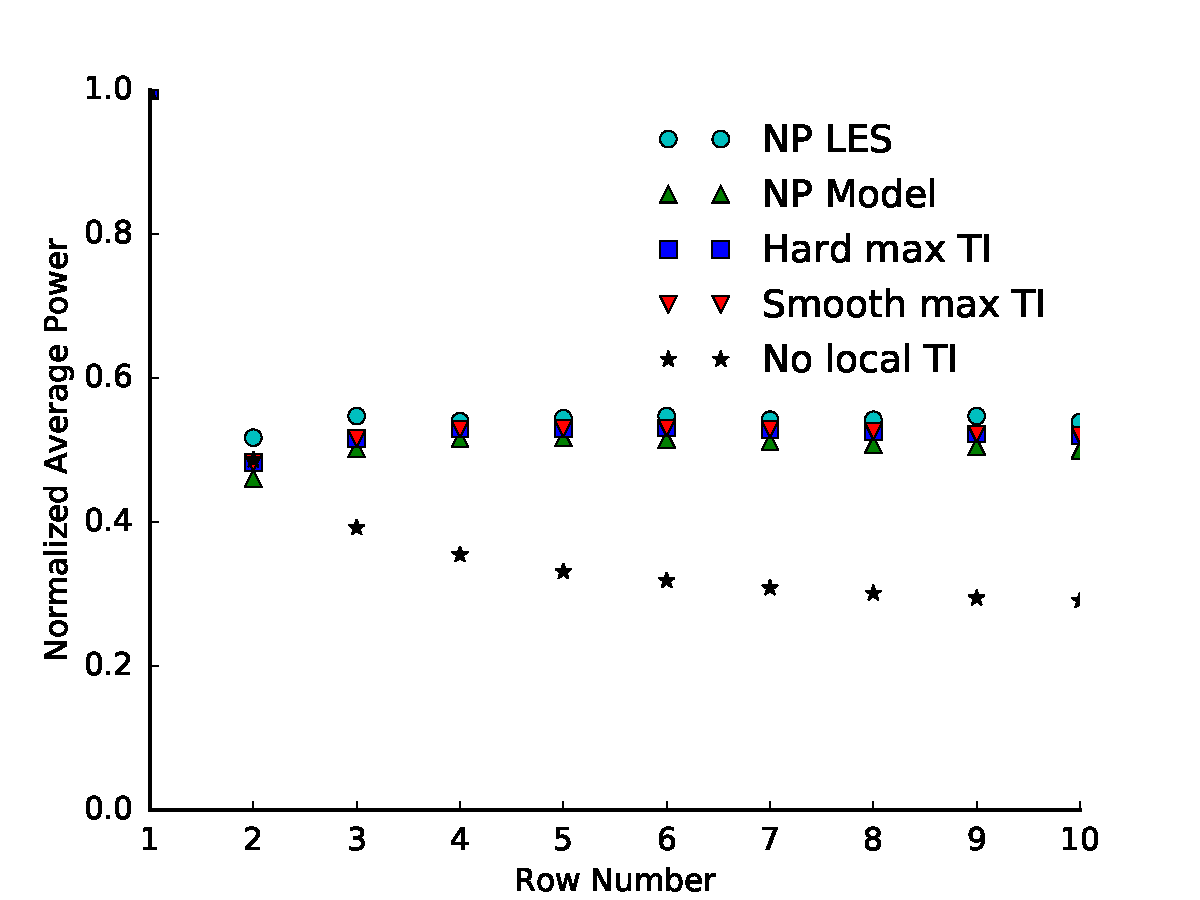
\includegraphics[width=0.48\textwidth, trim={0cm 0cm 0cm 0cm}]{final_images/power_by_row_horns_rev_100rpt.pdf}
	}
	\subfigure[]{
		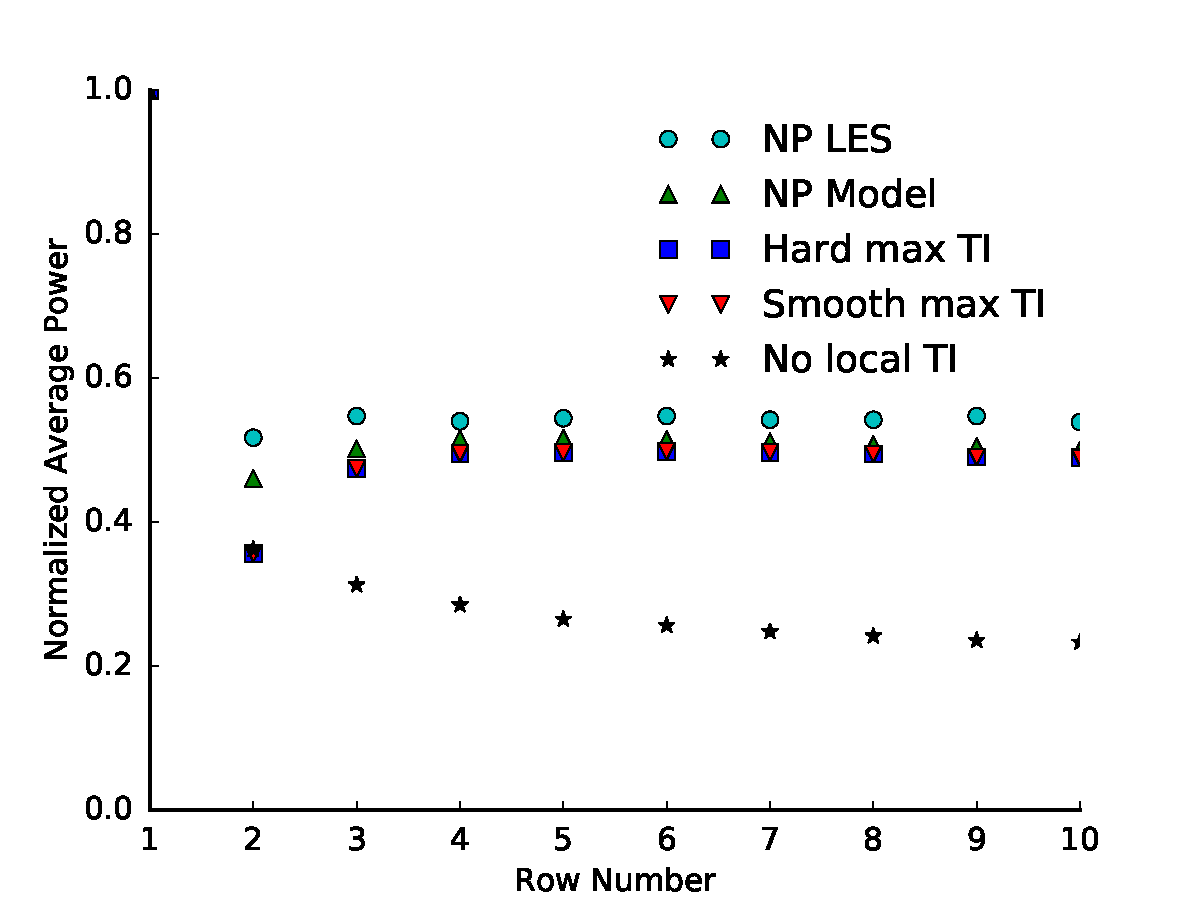
\includegraphics[width=0.48\textwidth, trim={0cm 0cm 0cm 0cm}]{final_images/power_by_row_horns_rev_1rpt.pdf}
	}
	\caption{Averaged power of turbines in columns two, three, and four of the Horns Rev wind farm by turbine row. NP refers to  data from \cite{niayifar2016}. (a) Comparing our code using 100 points to approximate the effective wind speed at the rotor. (b) Comparing our code using a single sample at the rotor hub to approximate the effective wind speed at the rotor.}
	\label{fig:power_line}
\end{figure}

\begin{figure}[htbp!]
	\centering
	\subfigure[]{
		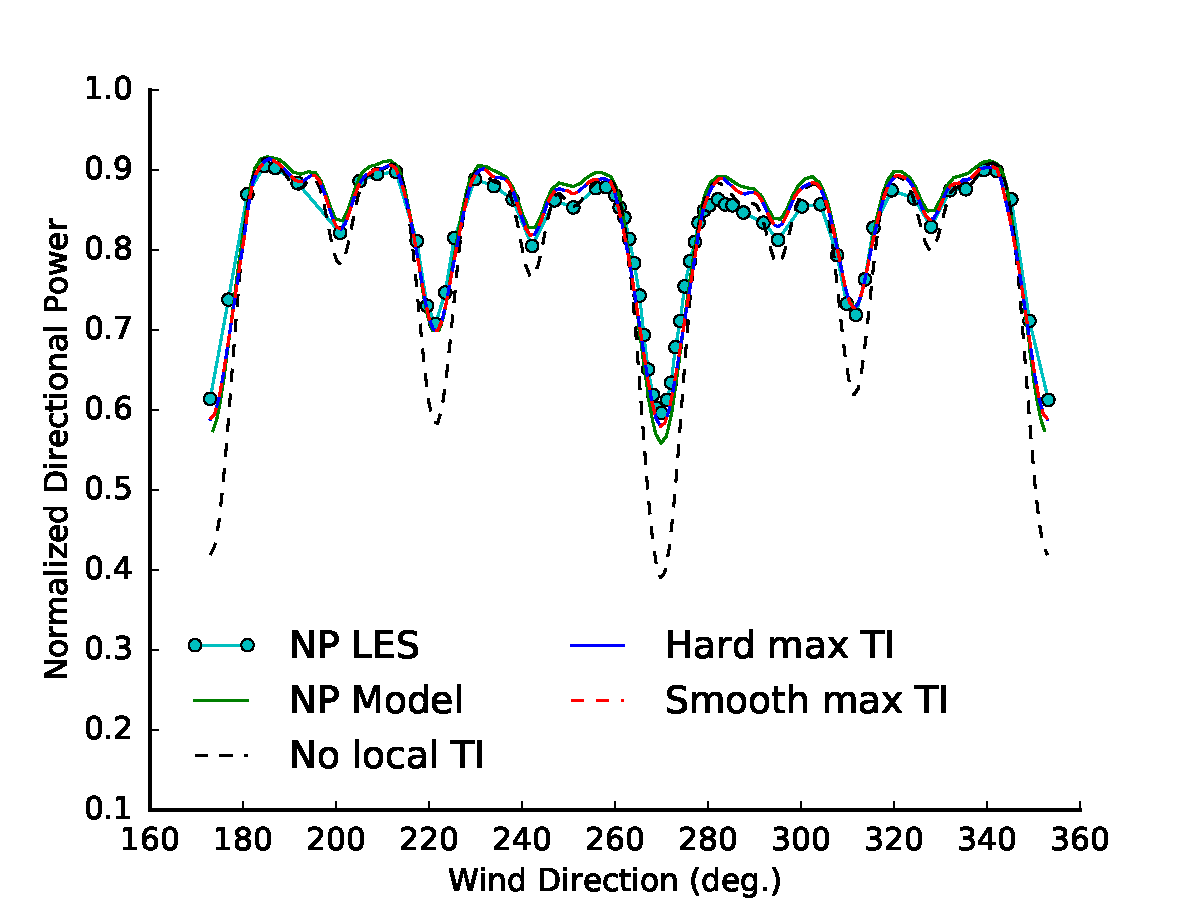
\includegraphics[width=0.48\textwidth, trim={0cm 0cm 0cm 0cm}]{final_images/power_by_dir_horns_rev_100rpt.pdf}
	}
	\subfigure[]{
		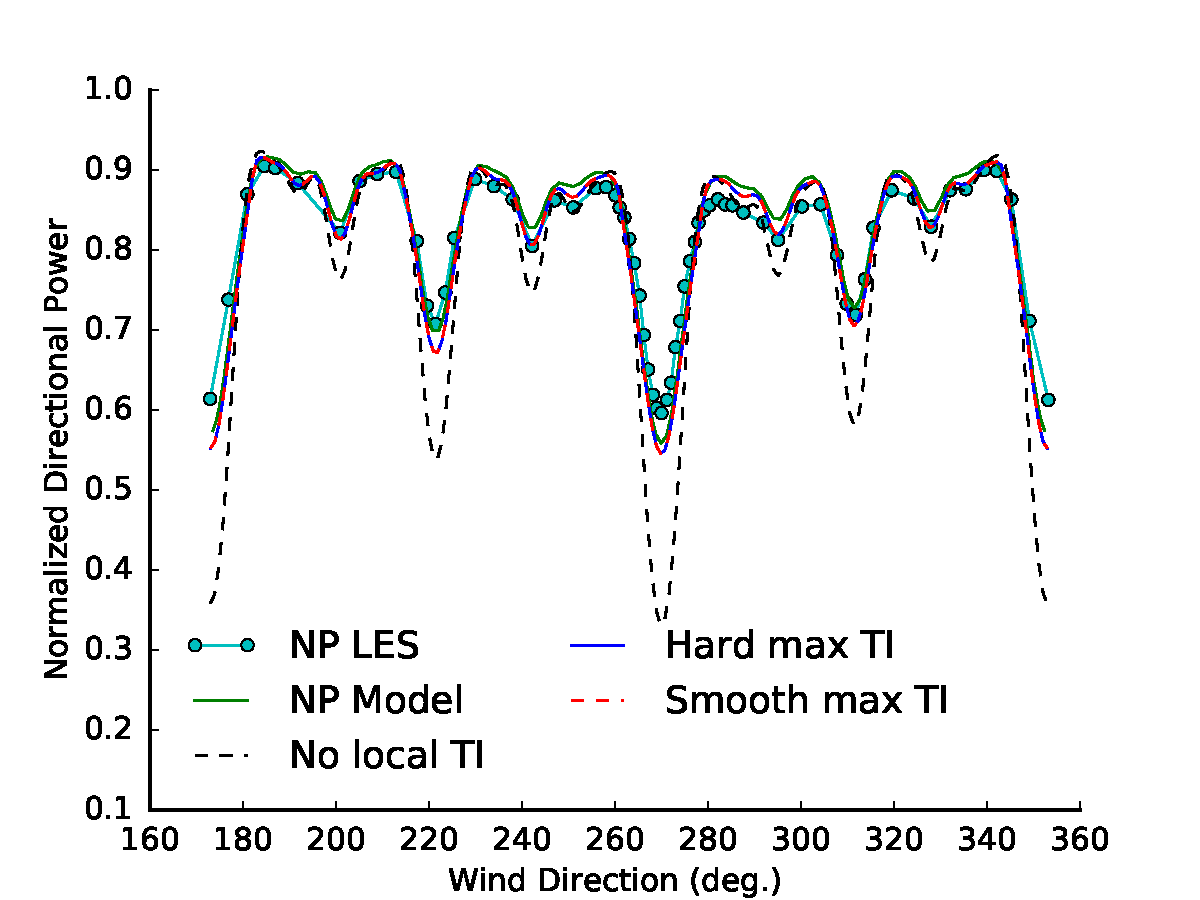
\includegraphics[width=0.48\textwidth, trim={0cm 0cm 0cm 0cm}]{final_images/power_by_dir_horns_rev_1rpt.pdf}
	}
	\caption{Power by direction for the Horns Rev wind farm. NP refers to data from \cite{niayifar2016}. (a) Comparing our code using 100 points to approximate the effective wind speed at the rotor. (b) Comparing our code using a single sample at the rotor hub to approximate the effective wind speed at the rotor.}
	
	\label{fig:power_direction}
\end{figure}

\subsection{Test Case}

For the LES validation, we used the NREL 5-MW reference turbine \cite{jonkman2009definition}. We used the same thrust and power coefficient curves for the NREL 5MW turbine as used in \cite{gebraad2017-max-aep}, with linear interpolation between points. Our test wind farm was constrained by the domain of the LES simulation precursor. We limited the LES simulation to an area 5 km square to keep necessary computational resources to a reasonable level. In order to avoid edge effects in the simulation, we needed at least 0.5 km between the edge of wind farm and the edge of the simulation space. To limit the computational cost, we used only a single wind direction and rotated the wind turbine locations within the simulation space to calculate the power production in different directions so that a single pre-cursor could be used. The resulting available space for the wind farm was a circle with a 2 km radius in the middle of the simulation space. Within the resulting circular region, we placed as many turbines as possible in a concentric circular pattern with a minimum allowable distance between turbines of 5 times the rotor diameter. The resulting layout is shown in \cref{fig:starting-layout}.    

\begin{figure}[ht]
	\centering
	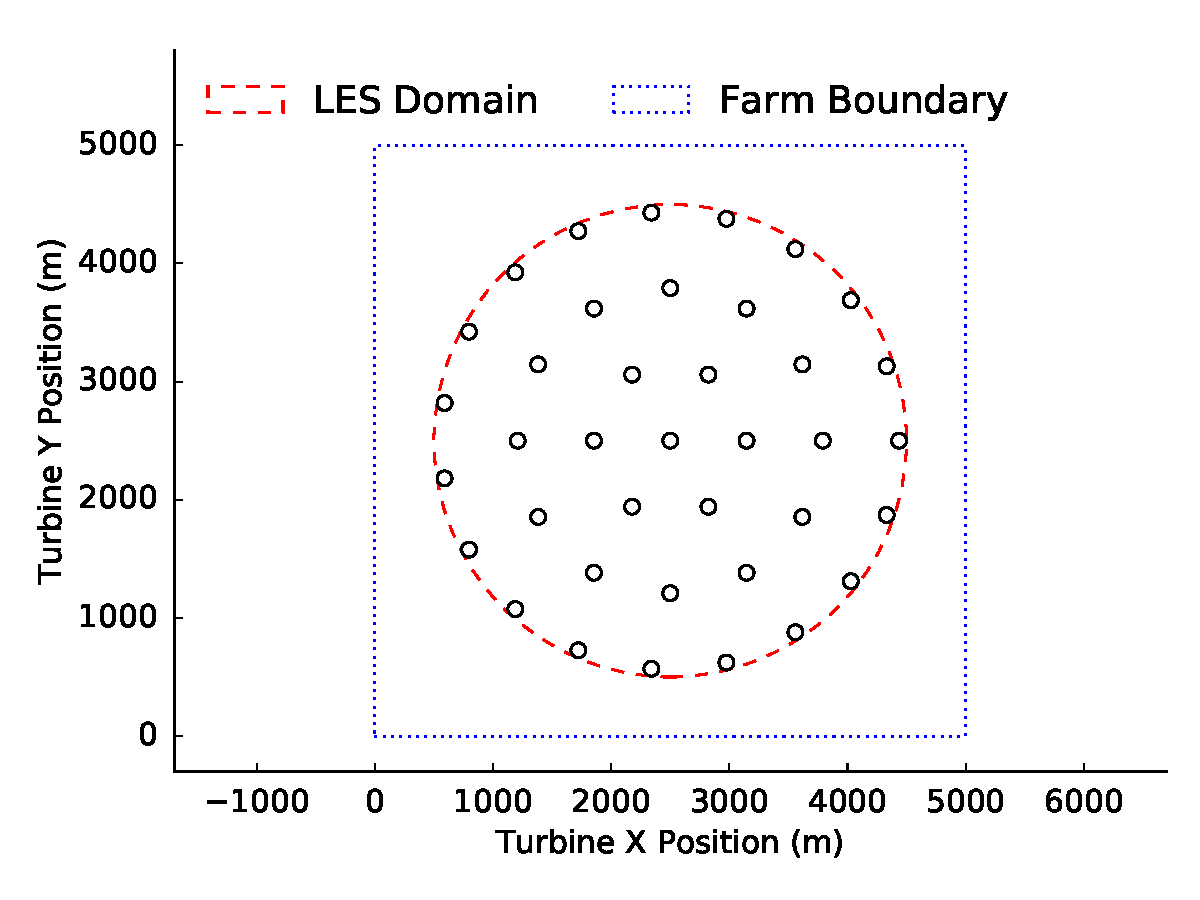
\includegraphics[width=0.75\textwidth]{final_images/round_farm_38Turbines_5DSpacing_start.pdf}
	\caption{Base case wind farm layout. The circles marking turbine locations are to scale, with diameters equal to the rotor diameter.}
	\label{fig:starting-layout}
\end{figure}

For the wind frequencies, we chose to use the Nantucket wind rose \cite{wrcc2017} %was selected as an approximation of the wind rose of the new Bay State Wind farm proposed for development off the coast of Massachusetts \cite{baystate2017}
. From this wind rose, 12 directions were selected by binning every 3 directions from the original wind rose starting with wind from the North. The original and final wind roses can be seen in \cref{fig:windrose}.

\begin{figure}[ht]
	\centering
	\subfigure[]{
		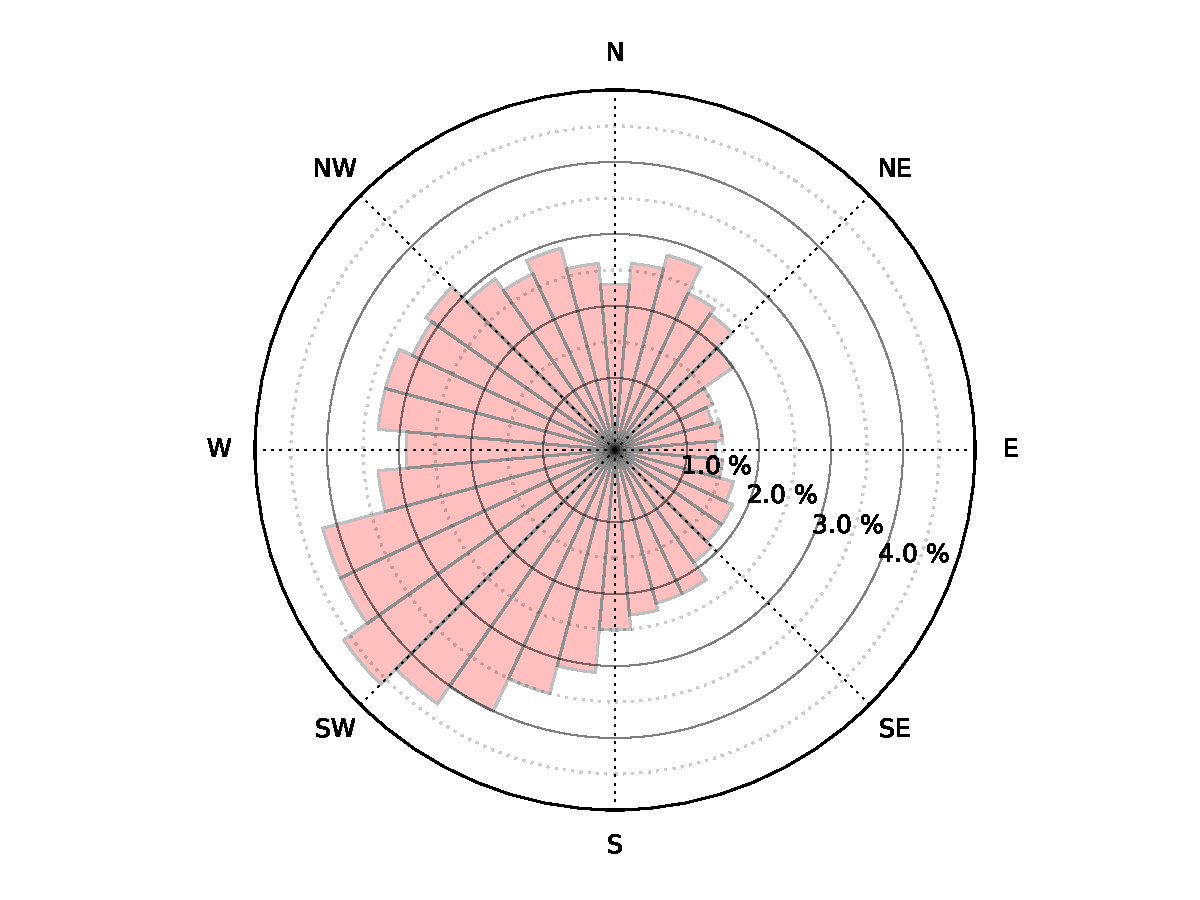
\includegraphics[width=0.48\textwidth, trim={3.25cm 0cm 3.25cm 0cm}]{final_images/windrose_full.pdf}
	}
	\subfigure[]{
		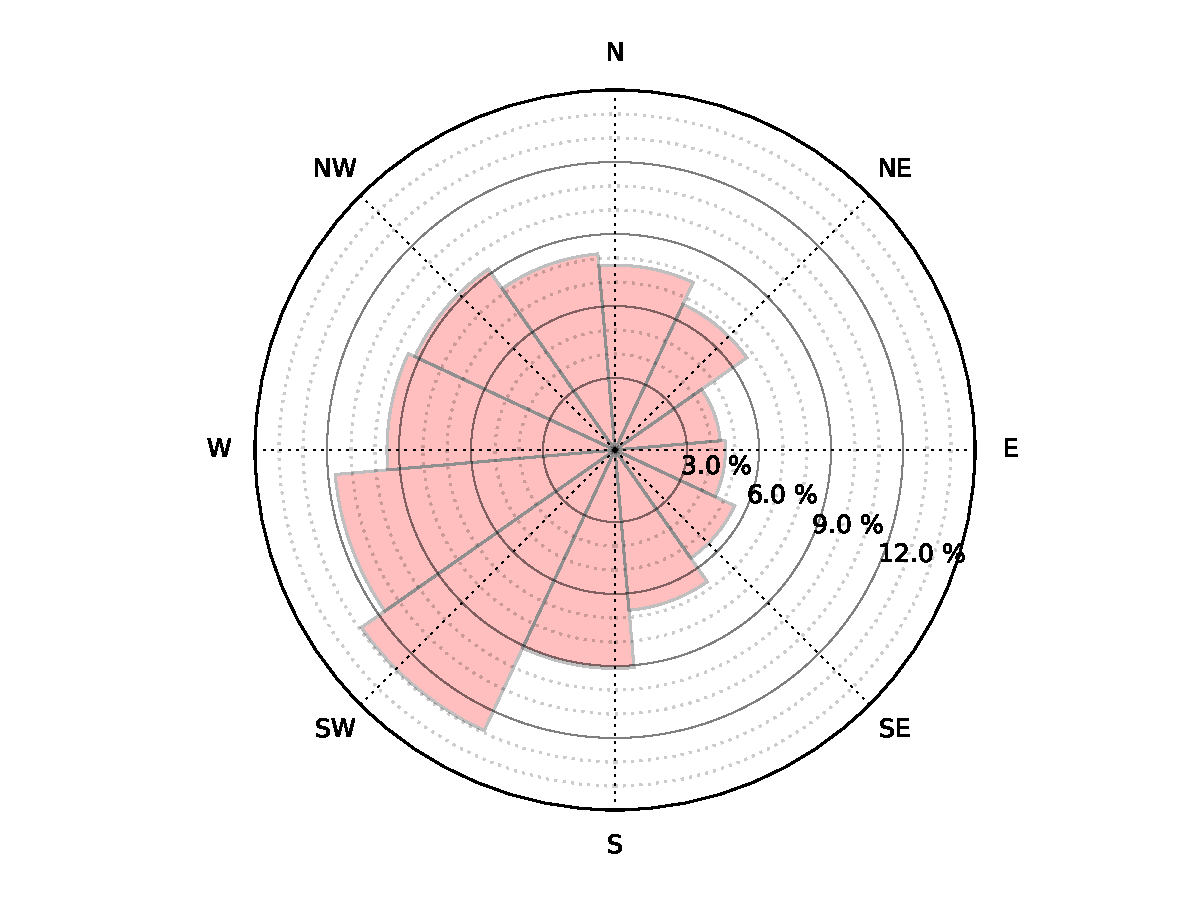
\includegraphics[width=0.48\textwidth, trim={3.25cm 0cm 3.25cm 0cm}]{final_images/windrose_les.pdf}
	}
	\caption{(a) Nantucket frequency windrose \cite{wrcc2017}. (b) Nantucket frequency windrose binned into 12 directions}
	\label{fig:windrose}
\end{figure}

\subsection{Optimization}

We optimized the layout using Annual Energy Production (AEP) as the objective. The optimization problem was formulated as
%
\begin{equation}
	\label{e:objective}
	\begin{aligned} [b]
	\underset{x_i,y_i}{\textrm{maximize}} \quad & AEP(x_i,y_i,)~~i=1...38\\
	\textrm{subject to} \quad & S_{i,j} \geq 2\*D_{r}~~i,j=1...38~~i \neq j\\
	 & [x_c-x_i]^2+[y_c-y_i]^2 \leq r_{b}^2~~i=1...38\\
	\end{aligned}
\end{equation}
%
Where $(x_i,y_i)$ is the position of each turbine $i$, $S_{i,j}$ represents the separation distance between each pair of turbines $i$ and $j$, $D_{r}$ is the rotor diameter, $(x_c,y_c)$ is the location of the center of the wind farm, and $r_b$ is the radius of the wind farm boundary.

The optimization problem was built in OpenMDAO, a Multidisciplinary Design Analysis and Optimization platform  \cite{gray2010_OpenMDAO}. Gradients of the wake model were obtained using Tapenade, an algorithmic differentiation tool \cite{tapenade2013}. Gradients of all other system components were derived by hand. The final system gradients were combined by OpenMDAO.

Once the problem was set up, it was scaled such that the gradients of both the objective function and constraints were close to order one. The final problem was then solved using SNOPT (Sparse Nonlinear OPTimizer), a gradient-based optimization algorithm that uses a sequential quadratic programming approach. SNOPT was used in this case because it is well suited to non-linear problems with high dimensionality \cite{gill2005}. 

We also used the Wake Expansion Continuation (WEC) method \cite{thomas2018-wec} with the following relaxtion factor values: $[3.00, 2.75, 2.50, 2.25, 2.00, 1.75, 1.5, 1.25, 1.00]$. We neglected local turbulence intensity during the WEC optimization series. After completing the WEC series, we ran one final optimization, from the optimized layout found using WEC. In the final optimization, local turbulence intensity was calculated with the smooth maximum function as in \cref{eq:smoothmax3}. The local turbulence intensity was ignored during WEC optimization because including local turbulence intensity introduces many more local optima in the design space that are exagerated by the use of WEC. 

To arrive at the final optimized solution, we optimized from the base case layout and 199 random layouts.
\subsection{Large Eddy Simulation}

\subsubsection{Simulator for Wind Farm Applications}

The simulator for wind farm applications (SOWFA) is a high-fidelity, large eddy simulation tool that was developed at NREL for wind plant studies \cite{churchfieldnwtc,churchfield2012numerical,fleming2013sowfa}.  It is a computational fluid dynamics solver based on OpenFOAM \cite{jasak2007openfoam} and can model turbines as actuator disks or actuator lines.  This study uses turbines modeled as actuator disks to reduce computational cost.  Separate studies have been conducted that demonstrate the steady-state power is similar in actuator disk and actuator line cases \cite{martinez2012comparison}.

SOWFA solves the three-dimensional, incompressible, Navier-Stokes euqtions and transport of potential temperature equations, which take into account the thermal buoyancy and Earth rotation (Coriolis) effects in the atmosphere.  The inflow conditions for these simulations are generated using a periodic atmospheric boundary layer precursor with no turbines.  

SOWFA calculates the unsteady flow field to compute the time-varying power, velocity deficits, and aerodynamic loads at each turbine in a wind plant.  This level of computation, with high-fidelity accuracy, takes on the order of hours to days to run on a supercomputer using a few hundred to a few thousand processors, depending on the size of the wind plant.  The simulations run for this study were performed on Peregrine, NREL's high-performance computer \cite{regimbal2015peregrine}.

It should be noted that studies have been performed to validate SOWFA.  For example, it has been compared with 48-turbine Lillgrund wind plant field data and shows good agreement through the first five turbines in a row aligned with the wind direction \cite{churchfield2012large}.  In addition, SOWFA has been tested to verify that it captures the inertial range in the turbulent energy spectra and log-layer in the mean flow, both of which characterize a real atmospheric boundary layer \cite{churchfield2012numerical}.  Further validation studies are ongoing.  

\subsubsection{Simulation Scenarios}

Actuator disk simulations of the 38-turbine layout described in the previous section were performed using SOWFA.  The turbines were simulated uisng the NREL 5\,MW reference turbine \cite{jonkman2009definition} at a 90.0\,m hub height and were operated in 12 different wind directions. To avoid running 12 different precursors, the layout was rotated to a reference wind direction of 270$^\circ$.  These scenarios were simulated under neutral atmospheric conditions with an 8\,m/s mean wind speed at hub height and approximately 6$\%$ turbulence intensity.  

Eachcase was set up and run in SOWFA.  The simulations each ran for approximately 2000\,s of simulated time.  A structured mesh is used in this study with grid spacings of 10\,m spacing in the $x$, $y$, and $z$ directions resulting in a grid that is 500 $\times$ 500 $\times$ 100, i.e. 25,000,000 grid cells.  Using 500 cores, simulations took on the order of 1 day to complete using actuator disk representations of the NREL 5MW turbine for each turbine.  

% \subsection{Comparing LES and Model Results}
% Comparison Approach

% Directional Power

% AEP

\section{Results and Discussion}

\subsection{Base Case Layout} \todo{fill in this section with LES comparison figures and discussion}
The 200 starting layouts' AEP is provided in \cref{fig:opt-distribution}.

\begin{figure}[ht]
	\centering
	\subfigure[]{
		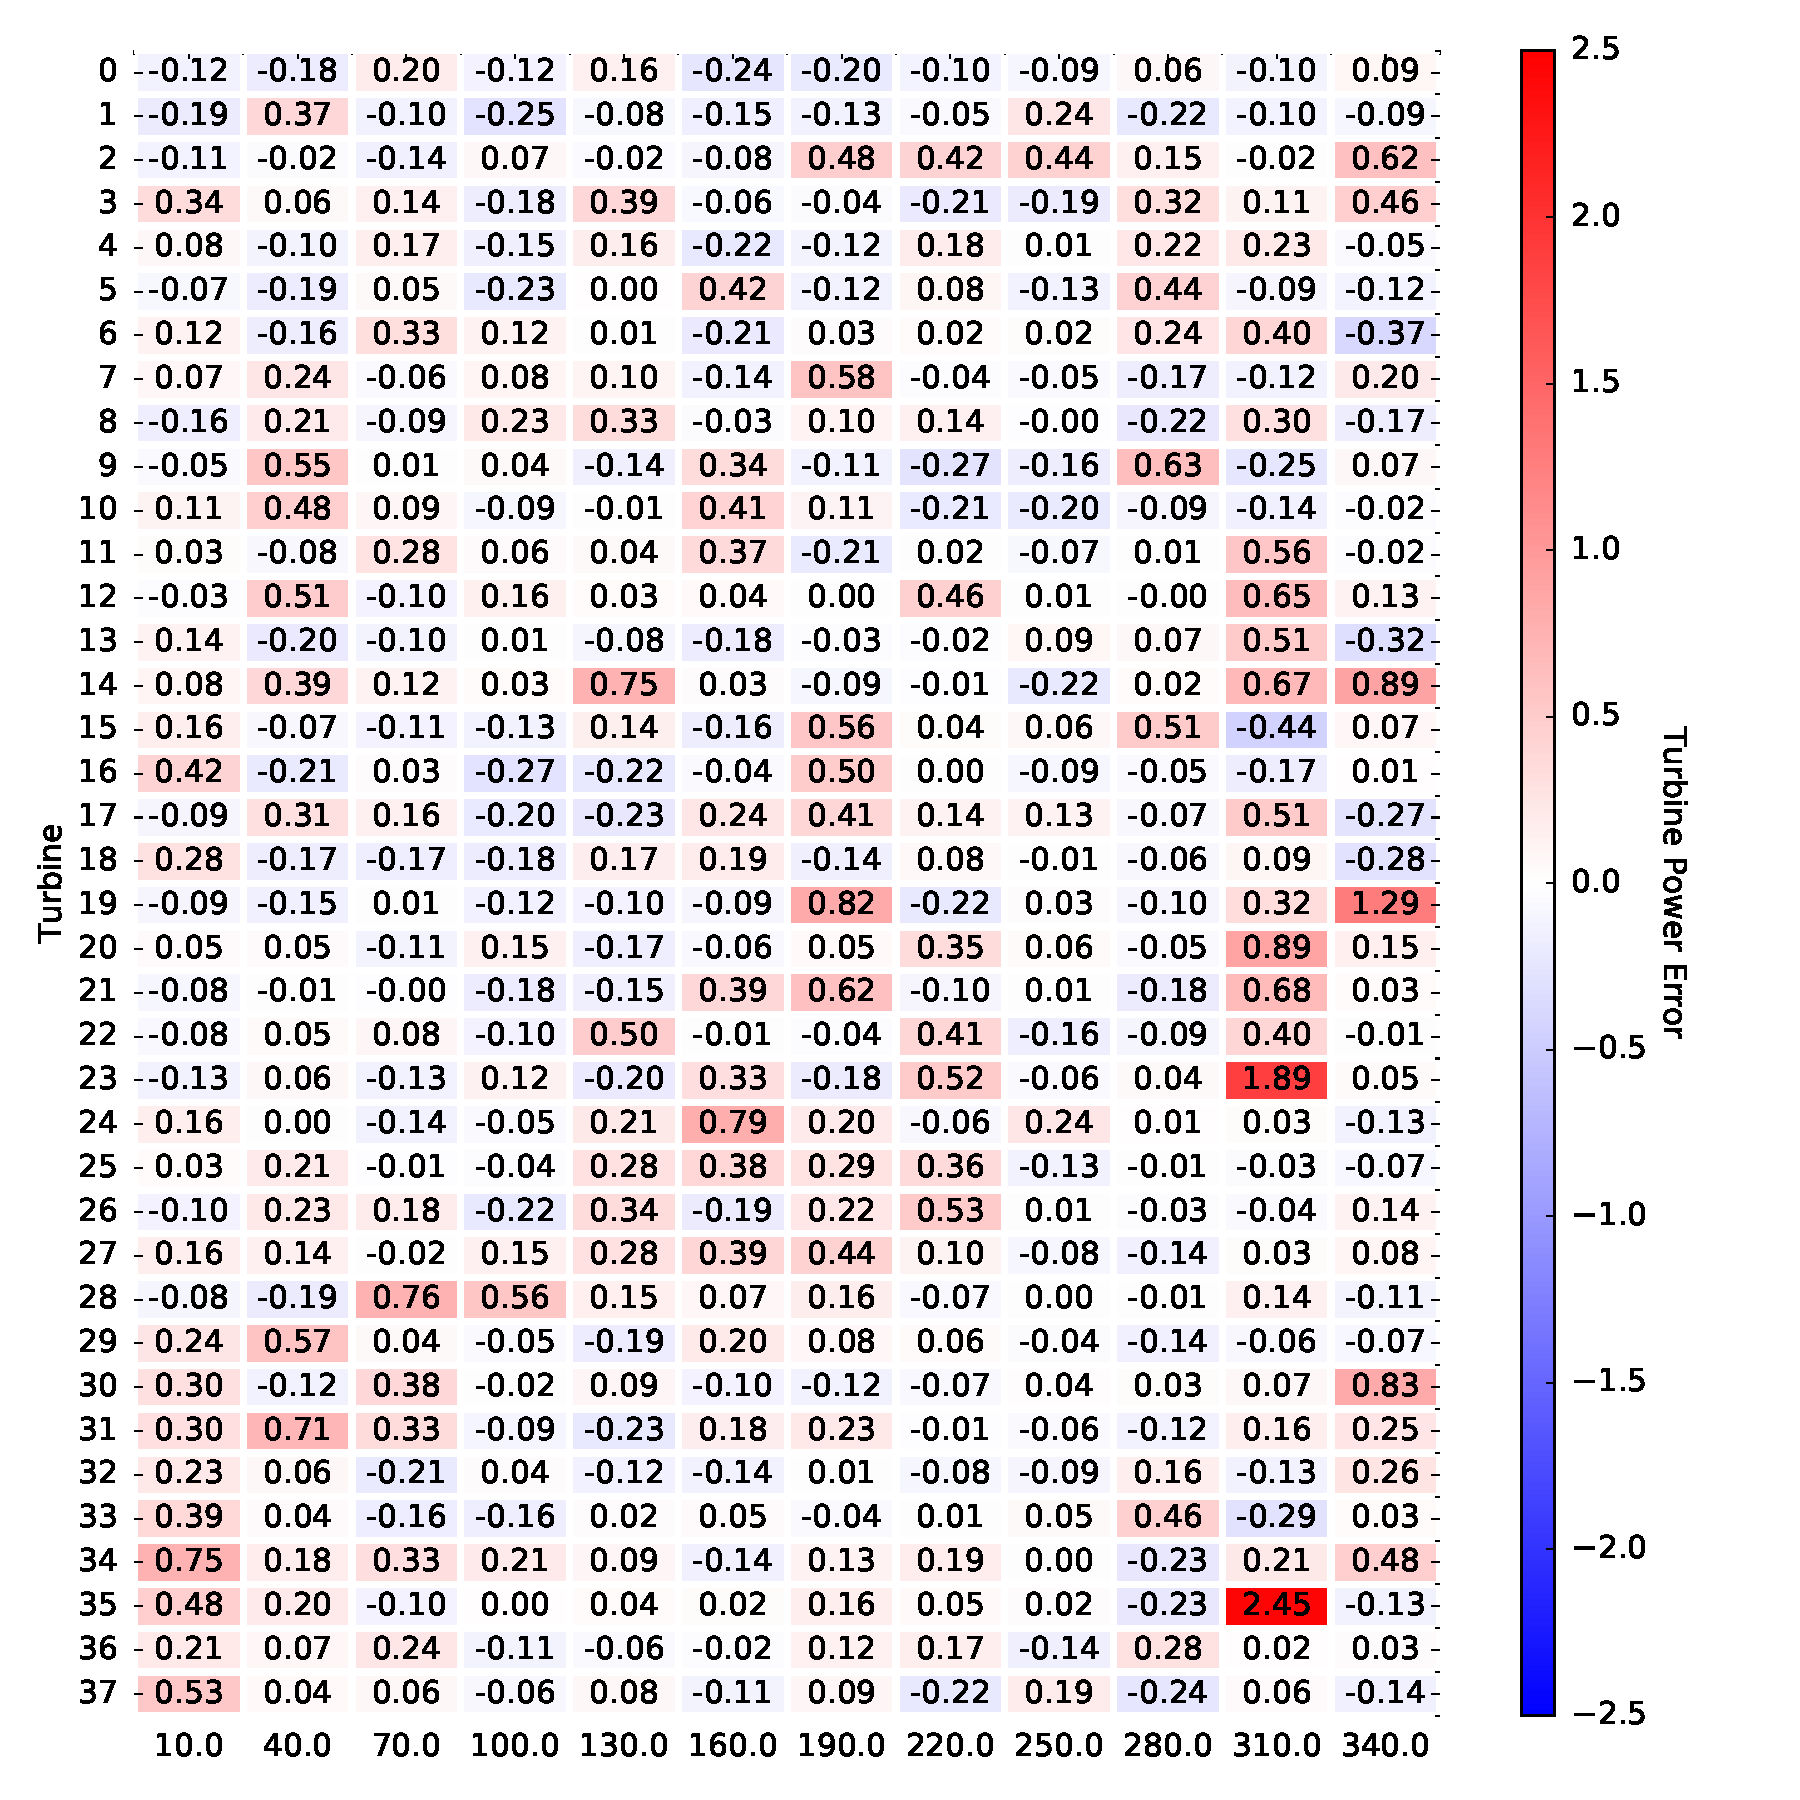
\includegraphics[width=0.98\textwidth, trim={0cm 0cm 0cm 0cm}]{final_images/sowfa_compare_pow_by_turb_dir.pdf}
	}
	\subfigure[]{
		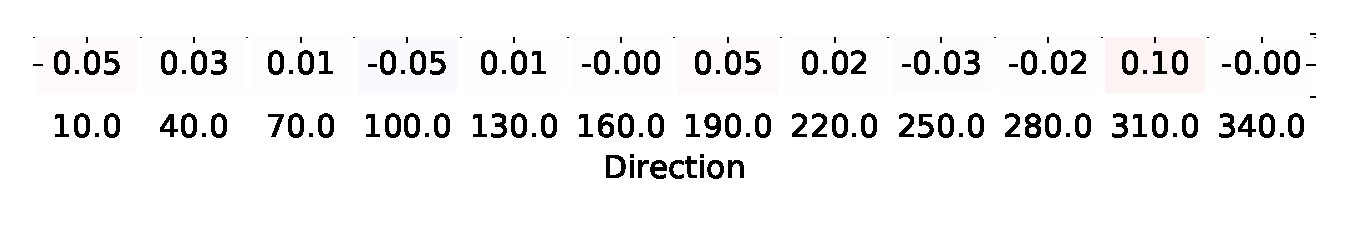
\includegraphics[width=0.77\textwidth, trim={1.75cm 0cm -1.75cm 0cm}]{final_images/sowfa_compare_pow_by_dir.pdf}
	}
	\caption{(a) Power production error of individual turbines in each direction as compared to SOWFA for the base case layout (\cref{fig:starting-layout}). (b) Directional power production error as compared to SOWFA for the base case layout (\cref{fig:starting-layout}).  The colorbar applies to both (a) and (b).}
	\label{fig:basecase-power-error}
\end{figure}

\subsection{Optimized Layout} \todo{re-outline this section}

\todo{re-write this section} The 200 starting layouts exhibited a distribution of results demonstrating the highly multi-modal nature of the WFLOP design space. The distribution of the optimization results can be seen in \cref{fig:opt-distribution}.
\begin{figure}[ht]
	\centering
	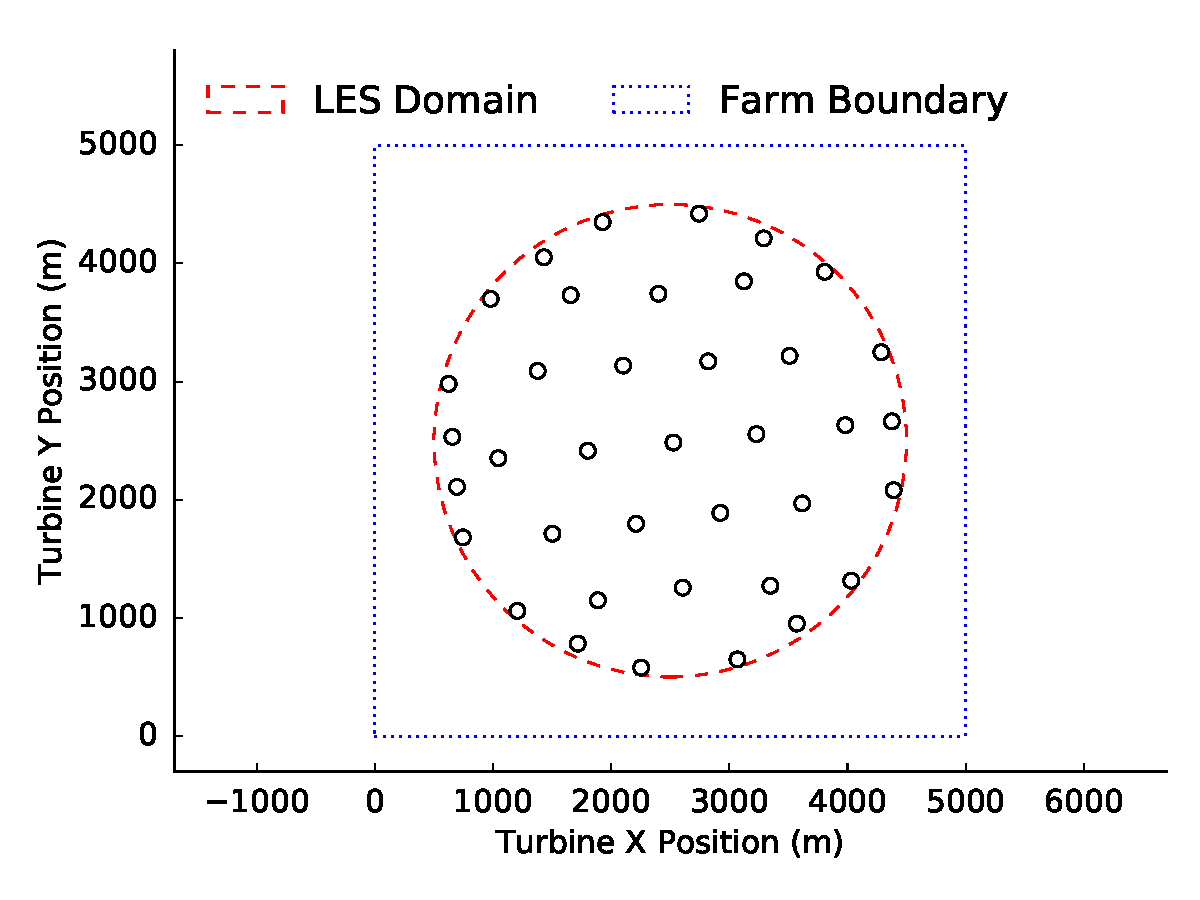
\includegraphics[width=0.75\textwidth]{final_images/round_farm_38Turbines_5DSpacing_finish.pdf}
	\caption{Optimized wind farm layout. The circles marking turbine locations are to scale, with diameters equal to the rotor diameter.}
	\label{fig:optimized-layout}
\end{figure}

\begin{figure}[ht]
	\centering
	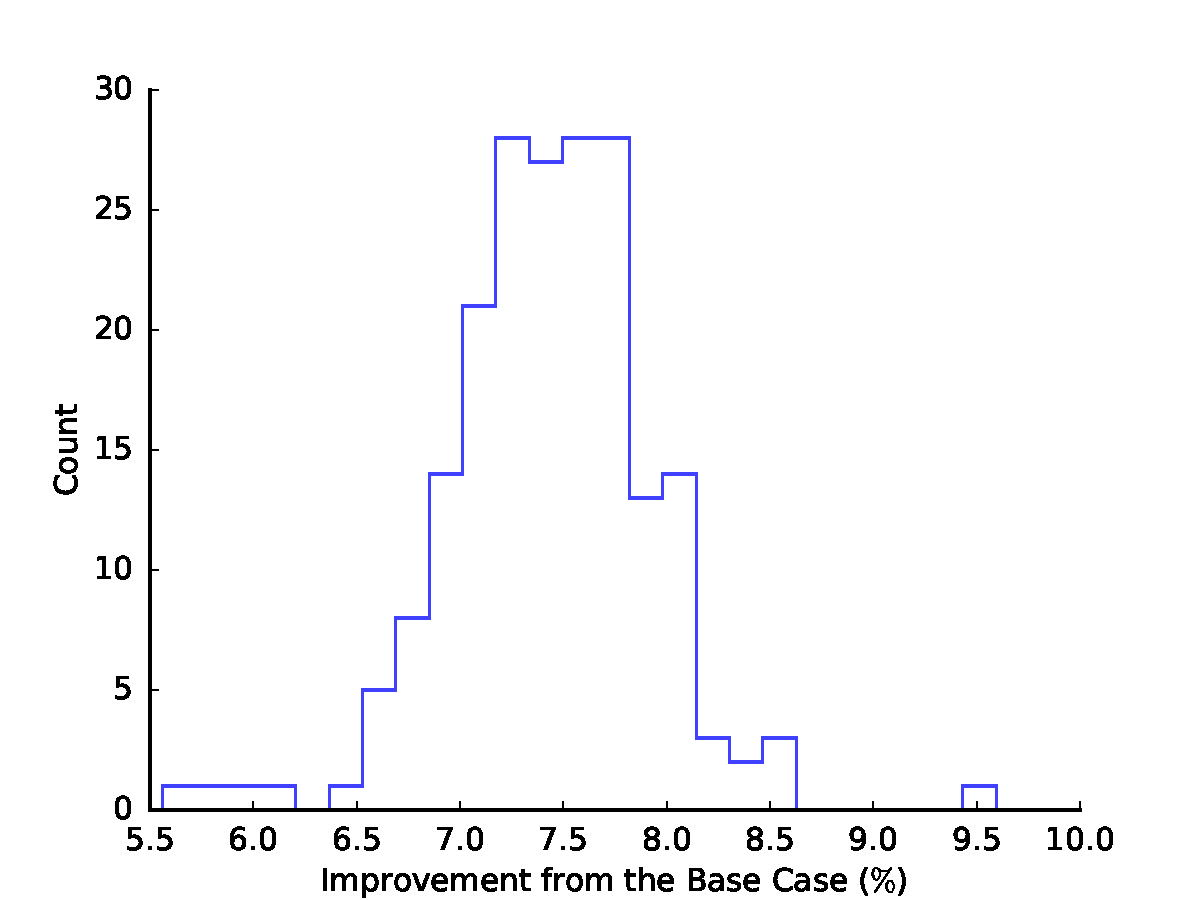
\includegraphics[width=0.75\textwidth]{final_images/38turbs_results_hist_aep.pdf}
	\caption{Distribution of optimized AEP results from the 200 optimization runs. The high outlier started from the baseline layout.}
	\label{fig:opt-distribution}
\end{figure}

Of the 200 starting layouts, the planned starting layout (shown in \cref{fig:starting-layout}) resulted in the highest AEP. 

\todo{outline LES methods and R\&D sections}
%The final layout with the highest AEP is shown in \cref{fig:final-layout}.

% \begin{figure}[ht]
% 	\centering
% 	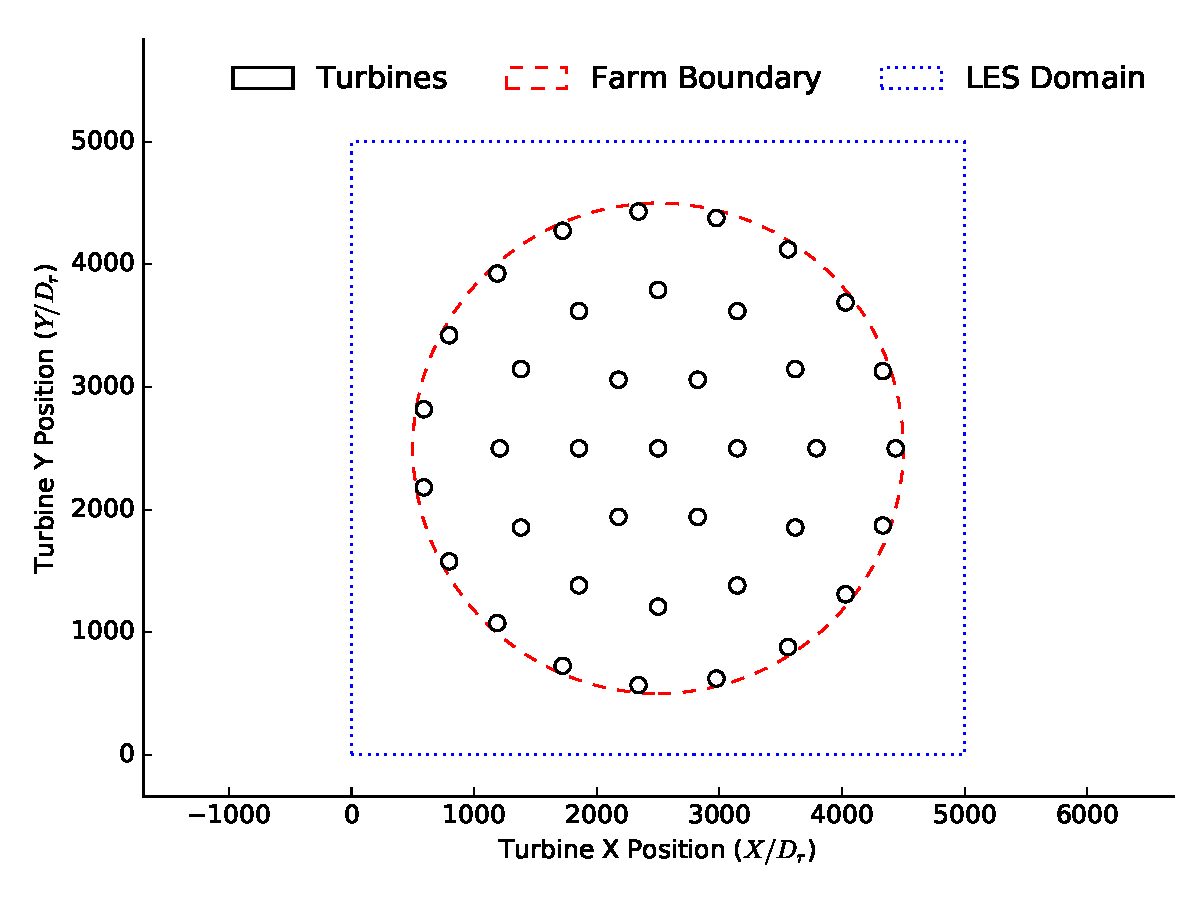
\includegraphics[width=0.75\textwidth]{final_images/round_farm_38Turbines_5DSpacing.pdf}
% 	\caption{Final optimized layout with the highest AEP. Obtained using the starting positions shown in \cref{fig:starting-layout}}
% 	\label{fig:final-layout}
% \end{figure}

% \subsubsection{Simplified Modeling}

% \subsubsection{LES Modeling}

% \subsubsection{Comparison}

% \subsection{Expected Results}
% We will run the each of the 12 wind directions using LES for both the base layout and the final optimized layout. To validate the results, we will compare the percent improvement in: total AEP,  directional power for each direction, and the power production of each individual turbine in each direction. The optimization results will be considered validated if the relative change from base to optimized layout at each level of granularity (i.e. AEP, direction, and turbine) for LES and the Bastankhah and Port\'{e}-Agel wake model are similarly significant and follow similar trends. We may also be able to determine how much of the improvement is real. We plan to provide bar charts, results tables, and other figures as appropriate.

%cases you plan to run, how you plan to use LES, the metrics you will use to compare (and what would be considered "validated"), etc.
% \section{Conclusion}
% This validation study will help us and other researchers understand how much of the improvement during optimization is real, and not an artifact of the models being used. This in turn will help us know how much improvement is needed based on simplified models to result in meaningful improvements to a real wind farm. 

\clearpage

\bibliographystyle{unsrt}
\bibliography{references/all_refs}
\end{document}